\documentclass[12pt,a4paper]{article}
\usepackage[utf8]{inputenc}
%\usepackage[hidelinks]{hyperref}
\usepackage{caption}
\usepackage{hyperref}
\usepackage{cite}
\usepackage[version=4]{mhchem} % for isotope symbols
\usepackage{a4wide}
\usepackage[lmargin=2cm,rmargin=2cm,tmargin=2cm,bmargin=2cm,headheight=0in]{geometry}
\usepackage{amssymb}
\usepackage{graphicx}


%\hypersetup{colorlinks, linkcolor={blue!50!black}, citecolor={blue!50!black},
%	urlcolor={blue!50!black}}
	
% Caption font sizes	
\DeclareCaptionFont{CaptionFontSize}{\fontsize{12pt}{12pt}}
\captionsetup[table]{font=CaptionFontSize}
\captionsetup[figure]{font=CaptionFontSize}

%Making bibliography compact
\let\oldbibliography\thebibliography
\renewcommand{\thebibliography}[1]{\oldbibliography{#1}
\setlength{\itemsep}{0pt}
\setlength{\parskip}{0pt}}

\newcommand{\cdm}{\ce{^{113\text{m}}Cd}}

\begin{document}
%\title{Nuclear isomers for energy storage and fundamental physics} - broad
%\title{Investigation of the energy storage potential of $\ce{^{113m}Cd}$ using time-correlated gamma ray-coincidence spectroscopy}% - narrower
%\title{Investigation of $\ce^{{113m}Cd}$ for energy storage and the physics of breakup in nuclear reactions} - narrowest
%\title{Investigation of $\ce{^{148,150,152}Ce}$ and $\ce{^{113m}Cd}$ using time-correlated gamma ray-coincidence spectroscopy}
%\title{Searching for octupole collectivity in neutron-rich Ce isotopes and isomer depletion pathways in $\ce{^{113}Cd}$} % Working title
%\author{Student: Caspian Nicholls (u1027945)}
%\date{Supervisor: Dr. A. J. Mitchell, Department of Nuclear Physics, Research School of Physics and Engineering, Australian National University}
%\date{\today}

\noindent
\textbf{Title: }Searching for octupole collectivity in neutron-rich Ce isotopes and isomer depletion pathways in $\ce{^{113}Cd}$

\noindent
\textbf{Author: } Caspian Nicholls (u1027945)

\noindent
\textbf{Supervisor: } Dr. A. J. Mitchell, Department of Nuclear Physics, Research School of Physics and Engineering, Australian National University

% From AJ
%Title: Probably needs to change. Something like “Search for octupole collectivity in neutron-rich Ce isotopes and isomer depletion pathways in 113Cd” ? 
%
%Context and aims: Opening paragraph to explain the situation of project change, then broader context. Set out the timeline of La decay analysis now until end of June. Reassess. Cd experiment ~ August (?) if possible. If this is set out clearly, then the rest can follow more easily. 
%

\section*{Context and Aims}

The initial focus for this project was to experimentally investigate the feasibility of storing energy using an excited state of the nuclide $\ce{^{113}Cd}$ with an exceptionally long half-life, known as a \textit{nuclear isomer} or \textit{metastable state}.
However, due to the global COVID-19 outbreak, the planned experiments can not be carried out at present.
If it becomes safe to perform these experiments at a time that still allows for a thorough analysis of the resulting data, returning to this research area shall be considered.
In the interim, the primary focus of this project is to analyse some yet unstudied experimental data and extend existing knowledge of the nuclear structure in the mass number A $\sim$ 144 region.

\medskip
\noindent
The primary reason isomers are worth investigating for energy storage applications is that the harnessable energy stored within nuclei is around $10^9$ J/g, approximately two orders of magnitude greater than that of chemical fuels.
Hence, isomers with half-lives above one year are currently being methodically studied to identify which of them could be used in energy storage devices with long lifetimes.
These devices would suit use in areas where the regular restocking of energy supplies may be impractical or inefficient, such as regions that are not easily accessible or highly remote~\cite{shaffer_innovations_2018}.

\medskip
\noindent
The isomer of $\ce{^{113}Cd}$ (denoted $\cdm$) has a half-life $T_{1/2} = 14.1$ years, making it a worthwhile candidate for such applications.
However, realising the potential of this metastable requires finding a mechanism by which the energy of the isomer can be released.
A current frontrunner is the process of \textit{isomer depletion}, where a nuclear isomer is excited into a more energetic state (an \textit{intermediate state} or \textit{depletion level}) that can then decay via a cascade of gamma rays into the ground state.
It has been demonstrated for isomeric forms of a small number of other isotopes, but not yet for $\cdm$~\cite{shaffer_innovations_2018}.

\medskip
\noindent
This investigation would be centered around constructing a picture of the excited states (\textit{level scheme}) of $\ce{^{113}Cd}$ and finding a sequence (\textit{depletion pathway}) of gamma ray transitions that connect the isomer to the ground state.
A secondary goal will be to explore the phenomenon of beam breakup (where the beam particle splits into smaller fragments that can each react with the target~\cite{curtis_+li_2005,dasgupta_fusion_1999}) using charged particle detectors, should they be functional when the experiments are performed.
The specific aims here would be to verify that beam breakup did occur and measure cross sections for reactions of each beam fragment with the target.


\medskip
\noindent
Yet, while access to the necessary experimental facilities is restricted, existing experimental data (consisting of gamma rays emitted by the excited states of neutron-rich isotopes $\ce{^{148,150,150}Ce}$) will be analysed.
These spectra were recorded during experiments designed to test the prediction of the deformed shell model of nuclear structure that nuclides with proton numbers Z near 56 and neutron numbers N near 88 will exhibit octupole collectivity.
This phenomenon denotes the collective motion of nucleons that causes the charge distributions of the excited states of these nuclei to deviate in geometry from the spherical shapes of their ground states.
As these nuclei comprise approximately 144 nucleons, one might expect that describing their collective motion might be quite complicated.
Hence, the fact that interactions between only a small number of the constituent nucleons are responsible for this behaviour is worth understanding.

\medskip
\noindent
At present, observations of these correlations have not been made for all of the nuclides predicted by the deformed shell model, including the neutron-rich isotopes $\ce{^{148,150,152}Ce}$.
Hence, the primary research aim of this project is to extend the existing body of information surrounding octupole collectivity in these A $\sim$ 144 nuclides.
% up to here

\medskip
\noindent
This will be achieved by analysing the recorded gamma rays to first construct a level scheme for these nuclides, including spectroscopic data (excitation energies, lifetimes, spins and parities) for the low-lying excited states.
Using this information, dipole and quadrupole moments of the charge distribution of the nuclei will be determined.
Identification of these moments will, in turn, allow deduction of the nature of any octupole collectivity that is present.%check

\medskip
\noindent
Regardless of this project's specific research focus, the underlying goal is to develop and utilise gamma ray spectroscopic analysis routines to extract key information from experimental nuclear data.
An aim that follows on from this is to meaningfully interpret this data under the framework of a range of theoretical nuclear structure models.

\medskip
\noindent
The latter aim above ties in with the ongoing experiments being performed by researchers to test the predictions of theoretical nuclear structure models and further our understanding of nuclear physics.
An understanding of this field has useful applications in astrophysics~\cite{hayakawa_neutron_2009}, energy storage~\cite{shaffer_innovations_2018}, nuclear medicine~\cite{krane_introductory_1987}, relativity and particle physics~\cite{casten_nuclear_1990}.



\section*{Background}
%Up to here 

\subsection*{Octupole correlations}
% Need to define octupole collectivity
The collective behaviour referred to by octupole collectivity can be described by considering the interaction of only a few nucleons because A $\sim$ 144 nuclides have Z and N near the closed-shell magic numbers Z = 50 and 82.
This means that within these nuclei, most nucleons form part of a frozen core that is largely unchanged when the nucleus is excited.
The nature of the excited state is thus determined by the few nucleons that become unpaired following the excitation (and the orbitals they occupy).

\medskip
\noindent
The observation of these interactions can provide evidence that a nucleus possesses a non-spherical (often pear-shaped) charge distribution.
These correlations arise when nucleons in nuclear orbitals with opposite parity (positive and negative) and a precise relationship between their quantum numbers interact strongly.
Specifically, the interacting orbitals will satisfy $\Delta n = 1$ and $\Delta l = \Delta j = 3$, where $n$, $l$ and $j$ denote the principal, orbital angular momentum and total angular momentum quantum numbers.
Based on the deformed shell model, near A $\sim$ 146, the proximity (in energy) of either the $h_{11/2}$ and $d_{5/2}$ proton orbitals or the $i_{13/2}$ and $f_{7/2}$ neutron orbitals (depending on the particular nature of the nuclear excitation) leads to octupole correlations because they satisfy the above relationships.
% Surely I don't need to explain the meaning of this orbital notation...

\medskip
\noindent
Previous, large arrays of gamma ray detectors have been used to record the gamma rays emitted by high spin excited states of neutron-rich nuclei  near $\ce{^{144}Ba}$ (Z $\sim$ 56, N $\sim$ 88) (formed from the spontaneous fission of $\ce{^{252}Cf}$) and study octupole collectivity~\cite{phillips_octupole_1988,chen_search_2006}.
Specifically, the observation of strong E1 transitions between the yrast sequences of energy levels with respectively positive and negative parities has provided much of the experimental evidence for octupole correlations near $\ce{^{144}Ba}$.
The description of these transitions as E1 provides information about the (orbital) angular momentum carried by the emitted radiation as well as its angular distribution~\cite{casten_nuclear_1990}.
% Don't think more detail is required here. If it is, I would say the following:
% The description of these transitions as E1 signifies that the emitted radiation carries an (orbital) angular momentum of $1$ in units of $\hbar$, has odd parity and has an angular distribution resembling the radiation from an electric dipole~\cite{casten_nuclear_1990}.
% It may not even be worth mentioning anything about what E1 (or XL in general) means at all.
The yrast sequence (or \textit{band}) of energy levels simply refers to that with the minimal excitation energy for a given value of the total angular momentum $J$~\cite{casten_nuclear_1990}.

\medskip
\noindent
Studies of low-spin states in nuclides near A $\sim$ 146 have also been made, by measuring the $\gamma$ rays emitted during the $\beta^-$ decays of $\ce{^{142,144,146}Cs}$ to obtain lifetime data for the low-spin states in the positive and negative parity yrast bands of $\ce{^{142,144,146}Ba}$~\cite{mach_influence_1990}.
A coincidence analysis method was used, wherein the time between the detection of a $\beta^-$ particle in one detector and a gamma ray in another gives the lifetime of the excited state populated when Cs $\beta^-$ decays into Ba.
This approach is valid because the time between the two particles being emitted is short enough that if they are detected sufficiently close together in time, they can be said to have originated from the same nucleus.
Collection of a sufficient number of these \textit{coincidence} events (so described because the detection of the two particles is effectively coincident) enables an accurate lifetime measurement.

\medskip
\noindent
Yet, relatively few studies of the isotopes $\ce{^{148,150,152}Ce}$ have been made, with most existing information on their level schemes coming from experiments that measured products of the spontaneous fission of $\ce{^{252}Cf}$~\cite{nica_notitle_117,
martin_notitle_114,
bazu_notitle_114}.
The experiments that generated the data to be analysed for this project were performed at the Californium Rare Isotope Breeder Upgrade (CARIBU) facility at Argonne National Laboratory (ANL).
At this facility, beams of neutron-rich (spontaneous) fission fragments of $\ce{^{252}Cf}$ such as $\ce{^{148,150,152}La}$ were transported to the low-energy CARIBU decay station and implanted on to the moving tape system.
This tape system periodically removes any sources with a long-lived activity that may obscure the signals of interest and is situated at the target position of the detector array.
This array contains four clover detectors (each comprising four Ge detectors) and between two and four LaBr(Ce) detectors, giving a total of (up to) 20 gamma ray detectors.
However, a plastic scintillator was also included in the detector array, specifically to detect $\beta^-$ particles.

\medskip
\noindent
These three detector types enable three-fold $\beta$-$\gamma$-$\gamma$ coincidence measurements to be made.
These in turn allow specific excited states to be identified and their lifetimes subsequently calculated.
The timing characteristics of the scintillator and LaBr(Ce) detectors used mean that this set up should enable measurement of excited state lifetimes as short as 30~ps.
These capabilities of the equipment used will thus ultimately enable the existing knowledge surrounding $\ce{^{148,150,152}Ce}$ to be extended, once the data is analysed.
% Is this sufficient detail on CARIBU?

%May need to include more background on octupole collectivity. See what AJ says.

\subsection*{Nuclear isomers}
In general, nuclear isomers exist because the decay of the isomeric excited state is inhibited.
This could be because the fundamental quantum mechanical selection rules for the allowed photon transitions between levels mean there are no lower energy states within that nucleus which the isomer may decay into.
Alternatively, the metastable state may only decay via transitions where the difference in the total angular momentum of the initial and final states $\Delta J$ (the \textit{multipolarity}) is relatively large.
This could account for the long lifetime of the isomer as transitions with large multipolarities are known to be slow relative to those with smaller $\Delta J$ values. 
Figure~\ref{fig:cd113} shows that $\cdm$ ($J = 11/2$, 263.54 keV) can only de-excite into the ground state ($J = 1/2$).
Thus it can only decay via a relatively high multipolarity $\Delta J = 5\hbar$ transition and falls into the latter category of isomer described above~\cite{blachot_notitle_111}.
\begin{figure}[htbp]
	\centering
	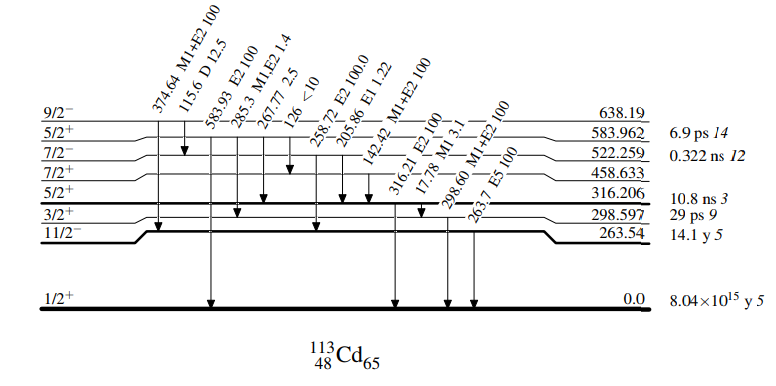
\includegraphics[width=0.9\textwidth]{113cd_partial_level_scheme_ENSDF.png}
	\caption{Partial level scheme for $\ce{^{113}Cd}$. The isomeric state has an energy of 263.54~keV~\cite{blachot_notitle_111}.}
\label{fig:cd113}
\end{figure}

\medskip
\noindent
Figure~\ref{fig:cd113} does suggest that there are already possible pathways by which $\cdm$ could be excited into a more energetic state and then decay into the ground state.
For example, the isomer could be excited into the $7/2^-$ state at 522.259~keV.
If it then decayed via an E1 transition to the 316.206~keV state before undergoing an E2 transition to the ground state, this would release the 263.54 keV stored in the isomer.
However, only 1.22 E1 transitions occur for every 100 E2 transitions from the $7/2^-$ state, so this pathway would not be strongly favoured and thus potentially not a reliable option for achieving isomer depletion. % check
There are other options within the level scheme of $\ce{^{113}Cd}$ shown in Figure~\ref{fig:cd113}, but they are each similarly flawed.
% Check this little tangent to make sure it is correct. Get AJ to pay attention to this when he reviews this proposal.

\medskip
\noindent
Yet, isomer depletion has been experimentally achieved for six other nuclides, using a range of distinct mechanisms.
These include exposing a sample containing a significant isomer population to bremsstrahlung radiation, using Coulomb excitation on another such sample, or initiating nuclear excitation by electron capture
~\cite{shaffer_innovations_2018}.
Thus, identification of a viable depletion pathway within $\ce{^{113}Cd}$ would extend the list of nuclides that can be harnessed to store energy over long timescales.
%Thus, should a practical depletion pathway be found within $\ce{^{113}Cd}$, these methods could be explored to demonstrate isomer depletion within this nuclide.

% Description of relevant models? Shell model, Nilsson/deformed shell model, ...?

\section*{Project Description}
%Project description: need to think about this
The analysis techniques and software that will be used are all methods and programs that are commonly used by and familiar to the other members of my research group.
They are also well documented, so there is a wealth of experience that can be tapped into when queries regarding the processing of data inevitably arise.
$\ce{^{148}Ce}$ and $\ce{^{150}Ce}$ have been studied using La $\beta^-$ decay experiments, so analysis of the recorded data for these isotopes will build on existing knowledge and potentially verify tentative conclusions reached in previous works.
Contrastingly, $\ce{^{152}Ce}$ has only been studied via the spontaneous fission of $\ce{^{252}Cf}$, so analysing this nuclide via the $\beta^-$ decay of $\ce{^{152}La}$ should provide new information on its structure.
Dedicated octupole collectivity studies have not been performed for any of these Ce isotopes, however, so this project will be breaking new ground in this area.
% Too grandiose?

\medskip
\noindent
By using $\beta$-$\gamma$ and $\beta$-$\gamma$-$\gamma$ coincidence analysis methods the program ROOT will be utilised to explore the recorded gamma ray data.
This process will enable the construction of a level scheme for each Ce isotope studied, aided by the consideration of $\gamma$-$\gamma$ coincidences (from the clover detectors) where one of the $\gamma$ rays is known to be emitted by a given Ce isotope.
Further analysis of gamma ray coincidences (as well as individual spectra) will then lead to the collection of key spectroscopic information, such as state lifetimes, excitation energies and spin-parities. %how for spin-parities?

\medskip
\noindent
If present, evidence of octupole collectivity will then be identified.
Primarily this will be achieved by looking for strong E1 transitions between yrast bands of opposite parity, which will naturally require identification of the yrast bands themselves.
% How do we identify the yrast bands?
The strength of the octupole correlations that are present will then be assessed by evaluating the dipole and quadrupole moments of different transitions.
% Check that this is right, and how this actually works... I have no idea
For each Ce isotope, this will result in the fabrication of a level scheme that will contain some new levels, transitions and spectroscopic information, as well as an assessment of the degree of octupole collectivity that they each exhibit.

% Be sure to justify the methods chosen more clearly, and explain how this work fits into the field. This also holds for the octupole collectivity part - done for now.
% Need to highlight that the octupole collectivity stuff is new/original (based on the research proposal for the experiments themselves) whilst the cadmium stuff is largely just trying to build on what has been done before - done for now.
\medskip
\noindent
As for the nuclear isomer phase of this project, isomer depletion-focused studies of $\ce{^{113}Cd}$ have not yet been recorded.
Hence, at the very least, these tests will build upon existing knowledge of the level scheme of this nuclide (and potentially the phenomenon of break up as well).
Some preparatory work for this phase has already occurred (Figure~\ref{fig:gantt}), including identifying the reactions to be used by reviewing previous experiments in the literature that focused on excited states of $\ce{^{113}Cd}$.
The qualitative behaviour of the relevant reaction cross sections as a function of energy has also been calculated using the PACE4 fusion-evaporation code.

\medskip
\noindent
Should this phase go ahead, the detectors to be used in the CAESAR gamma ray detector array will need to have their energy resolution characterised before being inserted into the array.
Simultaneously, calculations will have to be performed to determine the parameters (beam energies, target thicknesses, exposure times) that are optimal for the production and detection of excited states of $\ce{^{113}Cd}$.
Next, the targets will have to be readied, the experiments performed and then the data analysed. 
This data analysis will entail the construction of a level scheme, followed by the identification of any possible isomer depletion pathways.
Aside from the construction of the CAESAR array, I will be in charge of ensuring these steps are completed, with the help of other members of the ANU Nuclear Spectroscopy group as required.

\medskip
\noindent
If time remains and charged particle detectors (fabricated and tested by other members of the Nuclear Spectroscopy group) are included in the CAESAR array, breakup reactions that may have happened during the irradiation phase of the experiment could be investigated.
This would extend the measured results of this project and would be interesting from a theoretical physics point of view, but is not required to explore isomer depletion.
However, if all of the other tasks above are completed, then a level scheme for $\ce{^{113}Cd}$ will be able to be constructed and potential depletion pathways identified. 
% May need to provide more detail about beam breakup and the cluster structures of 7Li (alpha + tritium) and 9Be (alpha + alpha + n)


\section*{Project Plan and Feasibility}
% Insert Gantt chart with approximate deadlines.
% Could even be as approximate as going by month and just listing things to happen each month
% Data should be able to be accessed (via the server) from Friday 10 April.
% Current deadline for getting access to the lab again is 26 June.
\begin{figure}[htbp]
	\centering
	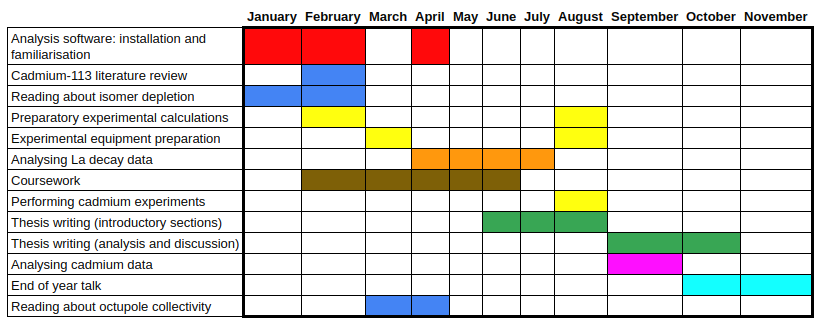
\includegraphics[width=0.9\textwidth]{GanttRP}
	\caption{Planned timeline for this project. The inclusion of experimental preparation and execution in August represents the latest feasible time when this can occur. Tasks assigned to January through March have been completed.}
\label{fig:gantt}
\end{figure}
% room to tweak this for sure

\medskip
\noindent
The time allocated to each of the following steps is outlined in Figure~\ref{fig:gantt}.
The following data processing steps are central to the completion of a satisfactory project and will be performed using the ubiquitous nuclear data analysis frameworks ROOT and Radware.
\begin{enumerate}
\item Check the energy and time calibration of the existing gamma ray data.
\item Analyse the data in ROOT to construct a level scheme for $\ce{^{148,150,152}Ce}$.
\item Establish excitation energies and lifetimes of excited states in $\ce{^{148,150,152}Ce}$.
\item Identify the multipolarities and transitions between excited states of $\ce{^{148,150,152}Ce}$.
\item Measure the lifetimes of the $\ce{^{148,150,152}La}$ ground states and constrain their spin-parities (stretch goal).
\end{enumerate}
%Write introduction, motivation, background and methodology sections of thesis. I expect to finish these by August 31.

\medskip
\noindent
These analysis processes shall be continued in a dedicated manner until September 1 at the latest.
Concurrent to this analysis the writing of the introduction, motivation, background and methodology sections of the thesis shall occur. 
As time progresses, we will assess the feasibility of completing the planned $\ce{^{113}Cd}$ experiments before September 1 weekly.
This date is the latest feasible point at which there will remain time for thorough data analysis, collation of results and completion of the thesis, all by October 29.

\medskip
\noindent
If restrictions on access to the required experimental facilities are lifted by August 1, then the steps below will be successively executed. The exact timing and feasibility will depend on beamtime being secured, through communication with my supervisor. All steps below are goals that are essential to the project unless otherwise specified.
%Dates somewhat arbitrary right now
\begin{enumerate}
\item Cool HPGe gamma ray detectors (for use in the CAESAR detector array) to liquid nitrogen temperatures.
\item Perform STROP calculations to identify the optimal target thickness, taking into consideration the energies identified as optimal for maximising the cross section for the reaction channel that produces $\ce{^{113}Cd}$.
\item Test HPGe detectors using PIXIE. Having already had some experience using this software, the completion of this step will not be a prolonged process.
\item Prepare $\ce{^{110}Pd}$ targets and create a mounting system for them. Establish whether we have enough targets and beamtime to perform experiments using both $\ce{^{7}Li}$ and $\ce{^{9}Be}$ beams.
\item Build the CAESAR detector array, in collaboration with A. J. Mitchell, Greg Lane, James Pope and other members of the Nuclear Spectroscopy group.
\item Perform experiments. Ideally, we would perform experiments with both $\ce{^{7}Li}$ and $\ce{^{9}Be}$ beams, but this is time and target dependent. If limited beam time is available, only one beam and a narrower range of beam energies may be able to be used.
\item Analyse data to construct a level scheme for $\ce{^{113}Cd}$ and identify any viable depletion pathways.
Deduce all possible spectroscopic information.
The analysis skills gained during the octupole collectivity part of the project will enable this to be completed efficiently.
\item Stretch goal: measure reaction cross sections as a function of energy.
\item Stretch goal: Investigate charged particle-$\gamma$ coincidence data to identify beam breakup reactions and measure their cross sections as a function of energy.
\item Write results, discussion and conclusion sections of the thesis, by October 29.
\item Prepare the final presentation, due November 5.
\end{enumerate}
This structure ensures that a satisfactory thesis will be generated from this project, but as it is the busiest possible timeline with all possible parts included, it provides plenty of room to omit aspects should the time no longer be available for them.
As a bare minimum, fundamentally interesting nuclear structure data be analysed and significant skills in the analysis of nuclear experimental data be developed, achieving the two primary goals of this project.
% probably need to explain the fact that there are many reaction channels and not all of them are desired.

%\vspace*{-\baselineskip}
\bibliographystyle{ieeetr}
\bibliography{references.bib}{}
% No more than 20 refs


\end{document}